\begin{figure*}[p]
\centering
\begin{subfigure}[t]{.95\columnwidth}
  \centering
  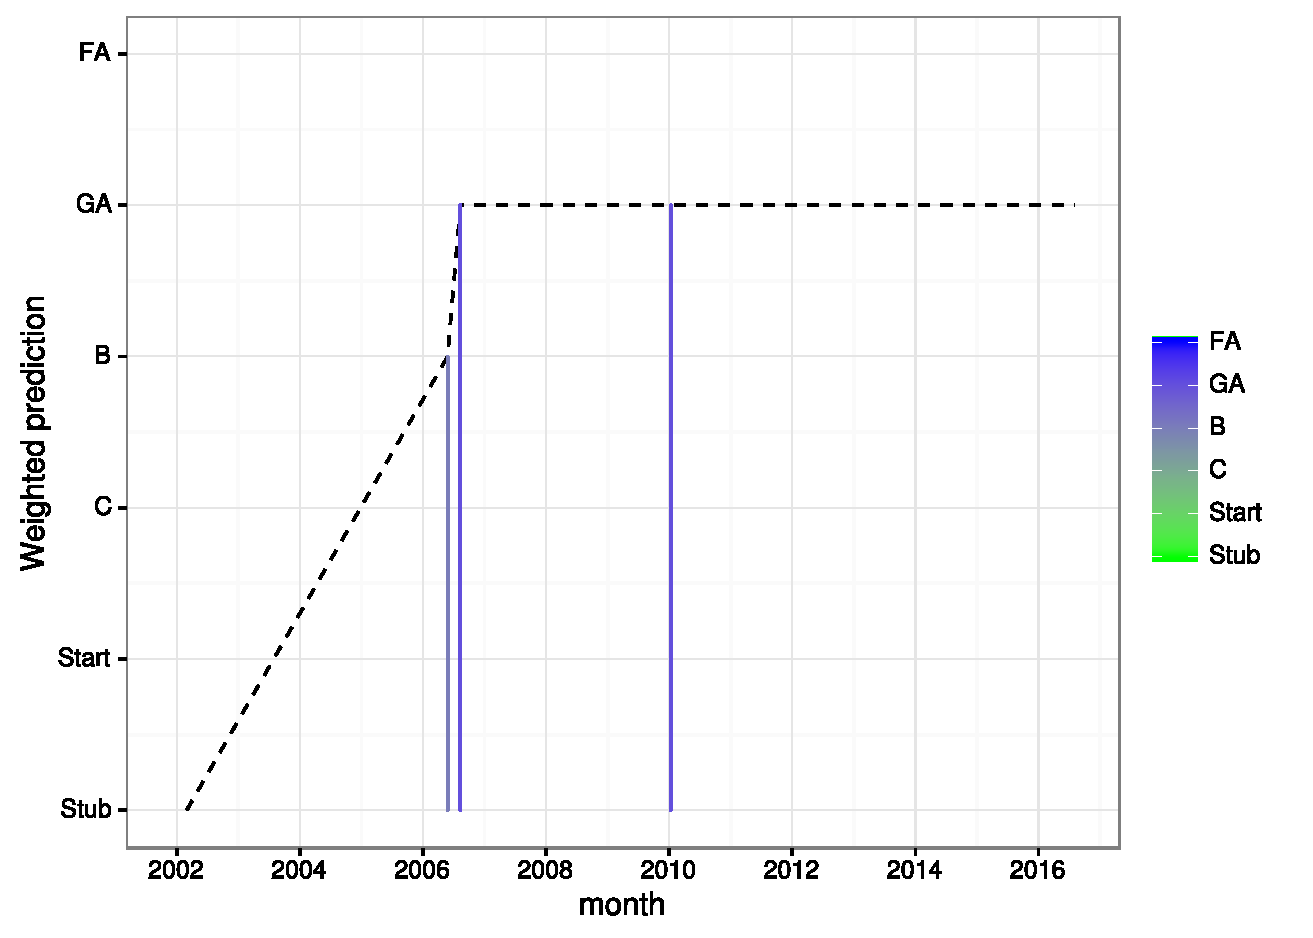
\includegraphics[width=.90\columnwidth]{figures/biology_monthly_assessments}
  \caption{Biology's assessments.  The 3 manual assessments of the quality of Biology are plotted over time with a dashed line connecting them.}
  \label{fig:empirical_biology}
\end{subfigure}~~
\begin{subfigure}[t]{.95\columnwidth}
  \centering
  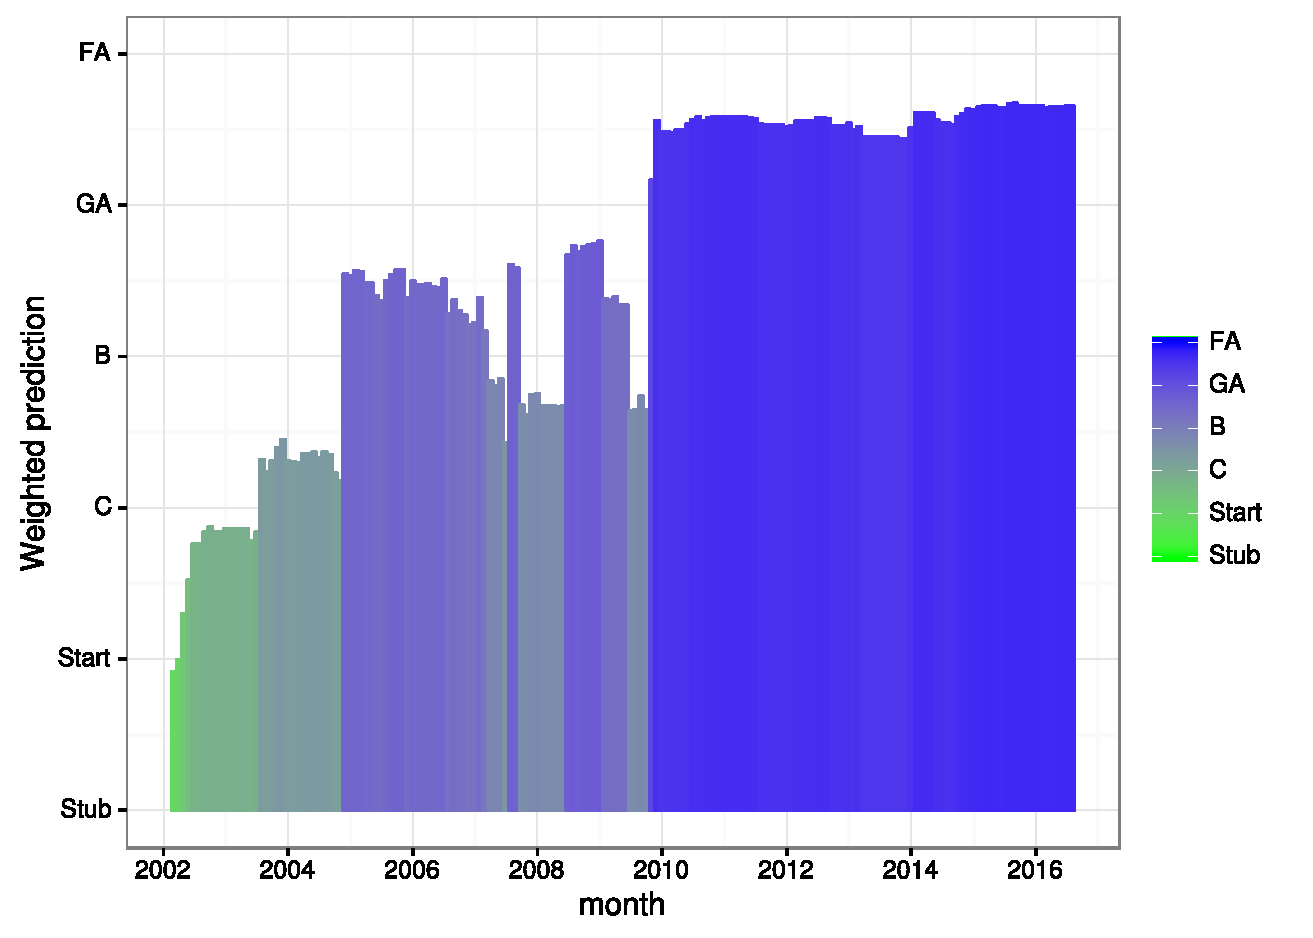
\includegraphics[width=.90\columnwidth]{figures/biology_monthly_wp10}
  \caption{Biology's predicted quality.  The \emph{weighted sum} prediction for the article Biology as of the last revision at the beginning of each month is plotted.}
  \label{fig:predicted_biology}
\end{subfigure}
\caption{Comparing assessments to predicted quality for Wikipepdia's article titled ``Biology''.  Note how~\ref{fig:predicted_biology} shows much more nuanced detail about the development of the article over time than~\ref{fig:empirical_biology}.}
\label{fig:empirical_and_predicted_biology}
\end{figure*}
